\subsection{Method's presentation}

\begin{figure}[!htbp]
	\centering
	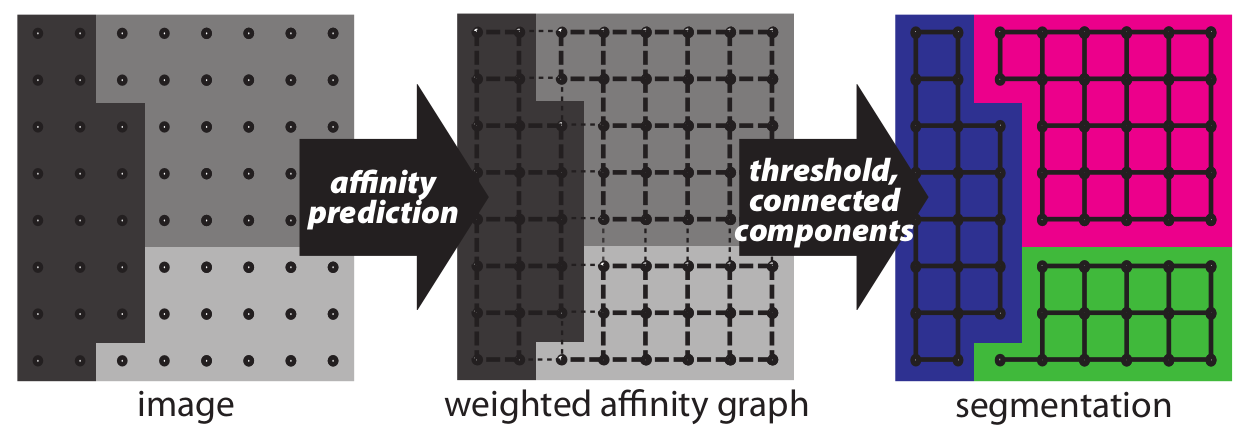
\includegraphics[width=0.8\linewidth]{./images/malis_method.png}
	\caption{Description of the method, from~\cite{turaga_maximin_2009}}%
	\label{fig:malis_method}
\end{figure}

The method, as illustrated in figure~\ref{fig:malis_method} works in two steps.\\
The first step is to compute an affinity graph $G$, with nodes $V$ representing
each pixel in the original image and edges $E$ weighted by the affinity between
neighbouring pixels. The graph $G$ will be 4-connected and for every pair of
pixels $i, j \in V\times V$ there exist and edge $(i,j)\in E$ if and only if $i$ and $j$ are
neighbours. We will note the affinity between neigbouring pixels $A_{ij}$.\\
An affinity of 1 between $i$ and $j$ means that they belong to the same object,
and an affinity of 0 means that they belong to different objects.\\

Once we have our affinity graph, with affinities between 0 and 1, we will
threshold it and remove edges under a certain affinity to obtain connected
components that will be our objects, and this thresholded affinity graph will
be our final segmentation.\\


\subsection{Optimizing the Rand Index}

There exist various methods of evaluating an image segmentation, one of them
being the Rand Index which is defined as follow :

\begin{gather*}
	1 - RI(\hat{S},S) = \binom{N}{2}^{-1} \sum_{i<j} \lvert \delta(s_i,s_j) -
	\delta(\hat{s}_i,\hat{s}_j) \rvert
\end{gather*}

With $S$ our groundtruth segmentation $\hat{S}$ our predicted segmentation and
$\delta(s_i,s_j)$ the indicator function taking value 1 if $s_i = s_j$ (if
pixels $i$ and $j$ are in the same segment/object) and 0 otherwise.\\
Intuitively, this can be seen as the fraction of image pixels where both
segmentations agree.

\begin{figure}[!htbp]
	\centering
	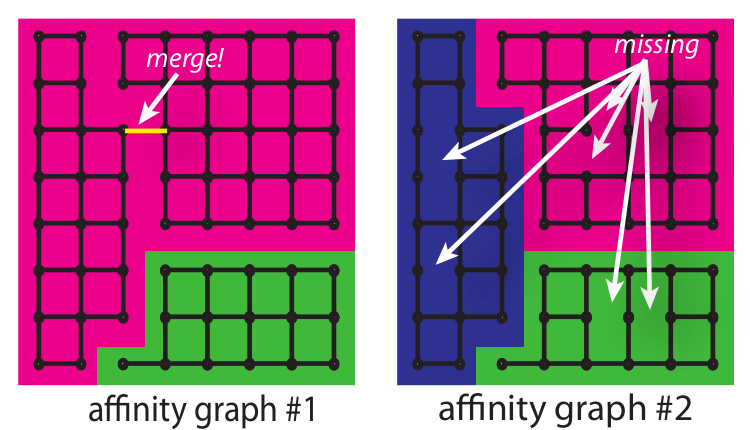
\includegraphics[width=0.45\linewidth]{./images/affinity_graphs.png}
	\caption{Example image segmentations and their affinity graph. On the left
	we have a merging of two objects due to a misclassified edge and on the
right we have edges that should be of value 1 that have been removed. From~\cite{turaga_maximin_2009}}%
	\label{fig:affinity_graphs}
\end{figure}

This gives us a way to evaluate an image segmentation that penalizes when two
objects are merged or split in our final segmentation as we can see in
figure~\ref{fig:affinity_graphs}. On the left, only one edge is misclassified
but this merges two objects and will be heavily penalized by the Rand Index (we
would see the same results if an object was split). On the contrary if we have
misclassified edges inside of objects that do not create any splits, this will
not be penalized at all by the loss since our objects are still correctly
delimited.\\

As such the Rand Index seems a good measure of segmentation quality for our
problem (edge-based segmentation). We will have to see how exactly we can
optimize this metric in our case.

\subsection{Maximin affinity and the maximin edge}

In order to optmize the Rand Index, we must find a way to compute
$\delta(\hat{s}_i,\hat{s}_j)$. To do this we will use the concept of maximin
affinity, as described in~\cite{turaga_maximin_2009}.\\
Let $\mathcal{P}_{ij}$ the set of all paths between $i$ and $j$ in our image.
For every path $P\in\mathcal{P}_{ij}$ there is an edge(s) $(k,l)$ with minimal
affinity.\\

This allows us to define the maximin path, which is the path which maximizes the
mininal affinity. It is defined as follow :
\begin{gather*}
	P^*_{ij} =\arg \max_{P\in\mathcal{P}_{ij}}\min_{(k,l)\in P} A_{kl}
\end{gather*}

The edge of minimal affinity in the maximin path will be called the maximin
edge and will be written $mm(i,j)$.\\
It allows to define the maximin affinity which is simply the affinity of the
maximin edge.
\begin{gather*}
	A^*_{ij} = \max_{P\in\mathcal{P}_{ij}}\min_{(k,l)\in P} A_{kl}
\end{gather*}

The most important consequence of this is that a pair of pixels $i,j$ is connected in
the thresholded affinity graph if and only if $A^*_{ij}$ is greater than the threshold
value, as shown in~\cite{turaga_maximin_2009}.\\

This means that if we can find the maximin affinity efficiently, we will be
able to compute the Rand Index efficiently.\\
In practice the maximin affinities can be computed efficiently using a maximum
spanning tree (MST), since any path in the MST is a maximin path.

\subsection{Computing an affinity graph}
As we can see, once we have our affinity graph, obtaining the segmentation is
straightforward, but the issue is : How to obtain an affinity graph? 

As stated before, an affinity graph is equivalent to the contours in the image,
and as such any method to find the contours in an image can be used to find the
affinity graph (with relative success).\\
The first idea that we could have would be to use a contour detector, such as
the Canny filter for example, however this would lead to an obvious over
segmentation, which is not desirable here.\\

An other idea (the idea used in~\cite{turaga_maximin_2009}) would be to use a
neural network to obtain our affinity graph. Neural networks, and particularly
convolutional neural networks (CNNs) have proven to be an extremely powerful
tool in image processing and especially in image classification and
segmentation, which makes them a good candidate for MALIS.\\

The architecture used originally is a fully convolutional neural network
(FCNN) which is a CNN with only convolutional layers. As such they can work
with various input sizes which is always a nice feature.\\

Now that we have seen how we can compute an affinity graph, let's see how we
can train this classifier, and if it is even possible to train it with the Rand
Index as a loss function.

\subsection{Training a classifier}

As stated before, the goal of this method is to optimize the Rand Index,
defined as:
\begin{gather*}
	1 - RI(\hat{S},S) = \binom{N}{2}^{-1} \sum_{i<j} \lvert \delta(s_i,s_j) -
	\delta(\hat{s}_i,\hat{s}_j) \rvert
\end{gather*}

with $S$ our groundtruth and $\hat{S}$ our predicted segmentation.\\
We can define $A^*_{ij}(I,\theta)$ the maximin affinity of pixels $i$ and $j$
in the predicted affinity graph of our classifier on $I$ with parameters
$\theta$. We can rewrite the previous equation as :
\begin{gather*}
	1 - RI(I,\theta,S) = \binom{N}{2}^{-1} \sum_{i<j} \lvert \delta(s_i,s_j) -
	 A^*_{ij}(I,\theta)\rvert
\end{gather*}

However this function is not differentiable everywhere so we cannot use it
directly for our training. We will replace the absolute value with a smooth
loss function $l$ such as the mean squared error. This relaxation will allow us
to use gradient descent to train our classifier(refer to~\cite{turaga_maximin_2009}
for more details on this).\\

Thus our final loss function will be :
\begin{gather*}
	L(I,\theta,S) = \binom{N}{2}^{-1} \sum_{i<j} l(\delta(s_i,s_j),
	A^*_{ij}(I,\theta))
	= \binom{N}{2}^{-1} \sum_{i<j} l(\delta(s_i,s_j),A_{mm(i,j)}(I,\theta))
\end{gather*}

We can now look at what the training loop will look like.

\begin{algorithm}
\begin{algorithmic}[1]
\caption{MALIS training loop, from~\cite{turaga_maximin_2009}}\label{alg:malis}
	\Repeat
		\State{Predict the affinity graph for an image $I$}
		\State{Pick two random pixels $i,j$ from $I$}
		\State{Find the maximin edge $mm(i,j)$}
		\State{Update our parameters $\theta$ with gradient}
		\begin{gather*}
			\nabla l(\delta(s_i,s_j),A_{mm(i,j)}(I,\theta)
		\end{gather*}
	\Until{convergence is reached}
\end{algorithmic}
\end{algorithm}

In practice we won't train on the whole image since it would be too long to
compute the maximin edge in the whole image. We will instead train on 21x21
patches of the image. We have to choose these patches carefully as most of them
will mostly be in an object and not around a border.\\
Since borders between objects are far less common than the "inside" of an
object, we may most of the time train only for pixels inside a same object.\\
This would result in class imbalance between our "borders" (affinity of value
0) and or "inside" (affinity of value 1). Training with such imbalance would
lead to worsened results since borders would not be present most of the time in
the chosen image (one example of such pathological behaviour would be the
prediction of affinity 1 everywhere, far from what we desire).\\

As such when training we need to be careful about what training image we
select.



